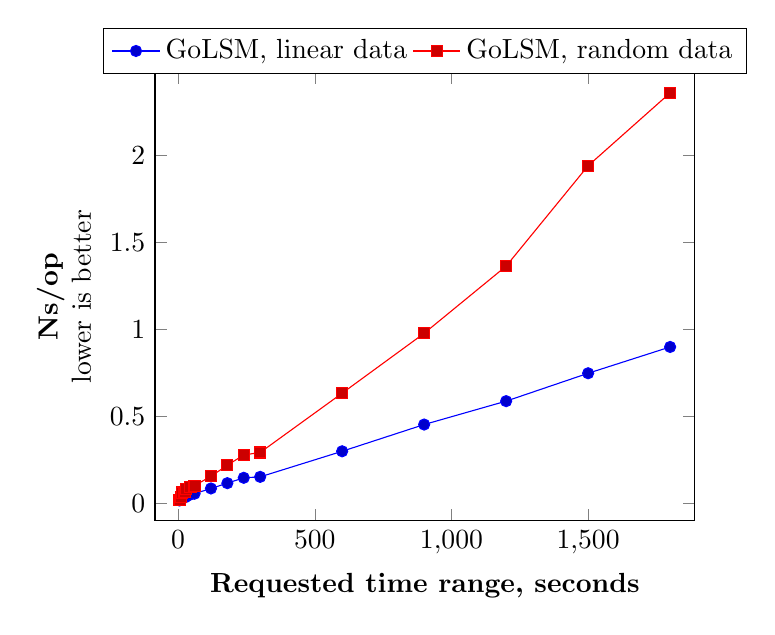
\begin{tikzpicture}
        % first provide your data as table, so later the data can
        % easily be accessed for various stuff
        \pgfplotstableread{
            x    y  z
5	15645901	20066750
10	22956983	34790230
15	32283634	61277403
20	34011973	66074549
25	33267746	63925416
30	39930080	83572878
45	49632256	94080339
60	54524124	100926498
120	84668307	154617448
180	115137807	218391345
240	146032654	277609792
300	151417281	291599762
600	298689957	633156270
900	452684093	977887157
1200	587385346	1364639379
1500	747870163	1942545058
1800	899311404	2362087783

        }{\data}
    \begin{axis}[
        x tick style={/pgf/number format/1000 sep=},
	    ylabel style={align=center},	
	    ylabel = \textbf{Ns/op}\\lower is better,
	    xlabel style={align=center},	
	    xlabel = \textbf{Requested time range, seconds},
	    enlargelimits=0.05,
	    legend style={
	        at={(0.5,1.1)}, anchor=north,legend columns=-1
	    },
    ]
        % then your `\addplot commands change to
        \addplot table [x=x,y=y] {\data};
        \addlegendentry{GoLSM, linear data}
        \addplot table [x=x,y=z] {\data};
        \addlegendentry{GoLSM, random data}
    \end{axis}
\end{tikzpicture}